\documentclass[titlepage, a4paper, 10pt]{article}

\usepackage{amssymb}
\usepackage{amsmath}
\usepackage{pgfplots}
\usepackage[margin=1in]{geometry}
\usepackage{fancyhdr}

\title{PLUS Session Worksheet \\[1em] \Large \textsc{Covering lessons: 1.3 -- 1.9}}
\date{May 25, 2023}
\author{MATH 1554}

% ------- Set up header -------
\renewcommand{\sectionmark}[1]{\markright{#1}} % from https://tex.stackexchange.com/a/317393/227665
\pagestyle{fancy}
\fancyhead[L]{\today}
\fancyhead[C]{\textit{\nouppercase{\rightmark}}}
\fancyhead[R]{\textbf{\thepage}}
% -------------------------------------------------------

% ------- Set up math stuff -------
\renewcommand{\vec}[1]{\mathbf{#1}}
\DeclareMathOperator{\vspan}{Span}
% -------------------------------------------------------

% ------- Set up Main Idea box environment -------
\newcounter{mainideas}
\setcounter{mainideas}{1}
\newcommand{\mainidea}{\textbf{Main Idea \#\themainideas \stepcounter{mainideas}}}
\setlength\fboxsep{1em}
%\newcommand{\midea}[2]{\begin{center}\fbox{\parbox{#1}{\centering \mainidea #2}} \end{center}} % Could be environment but I couldn't bother

% The way this works is that the savebox collects whatever was between the minipage and the end of it, then in the last line of the definition of the environment
% we regurgigate whatever was collected into an fbox which we center.
\newsavebox{\mybox}
\newenvironment{mideea}[1]
{%
\begin{lrbox}{\mybox}%
	\begin{minipage}{#1\textwidth}
		{\centering \mainidea \par}

}
{\end{minipage}\end{lrbox}\begin{center}\fbox{\usebox{\mybox}}\end{center}}
% -------------------------------------------------------

% ------- Set up activity environment -------
\newcounter{activity}
\setcounter{activity}{1}
\newenvironment{newactivity}
{
	\noindent\textbf{Activity \theactivity}
}
{
\stepcounter{activity}
\par
}
% -------------------------------------------------------

% Loner, from the overleaf website
\pgfplotsset{compat=1.9}

\begin{document}
\maketitle

\section{\centering Span \& Vector Equations (1.3)}

\subsection{Span}
\begin{mideea}{0.9}
	For \(\vec{v}_1, \vec{v}_2, \dots, \vec{v}_n \in \mathbb{R}^n:\)
	\[\vspan \{\vec{v}_1, \vec{v}_2, \dots, \vec{v}_n\} = \{c_1\vec{v}_1 + c_2\vec{v}_2 + \dots + c_n\vec{v}_n \mid c_i \in \mathbb{R}, 1 \le i \le n\}\]
	\centering \textit{The span of a set of vectors is the set of all possible linear combinations of those vectors.}
\end{mideea}

\begin{newactivity}
Sketch the span of: 
	\begin{enumerate}
		\item A set of 1 vector whose span forms a line.
		\item A set of 2 vectors whose span forms a line.
		\item A set of 2 vectors whose span forms a plane.
	\end{enumerate}
\end{newactivity}
\begin{figure}[!h]
\centering
	\begin{minipage}{0.3333\textwidth}
	\centering
	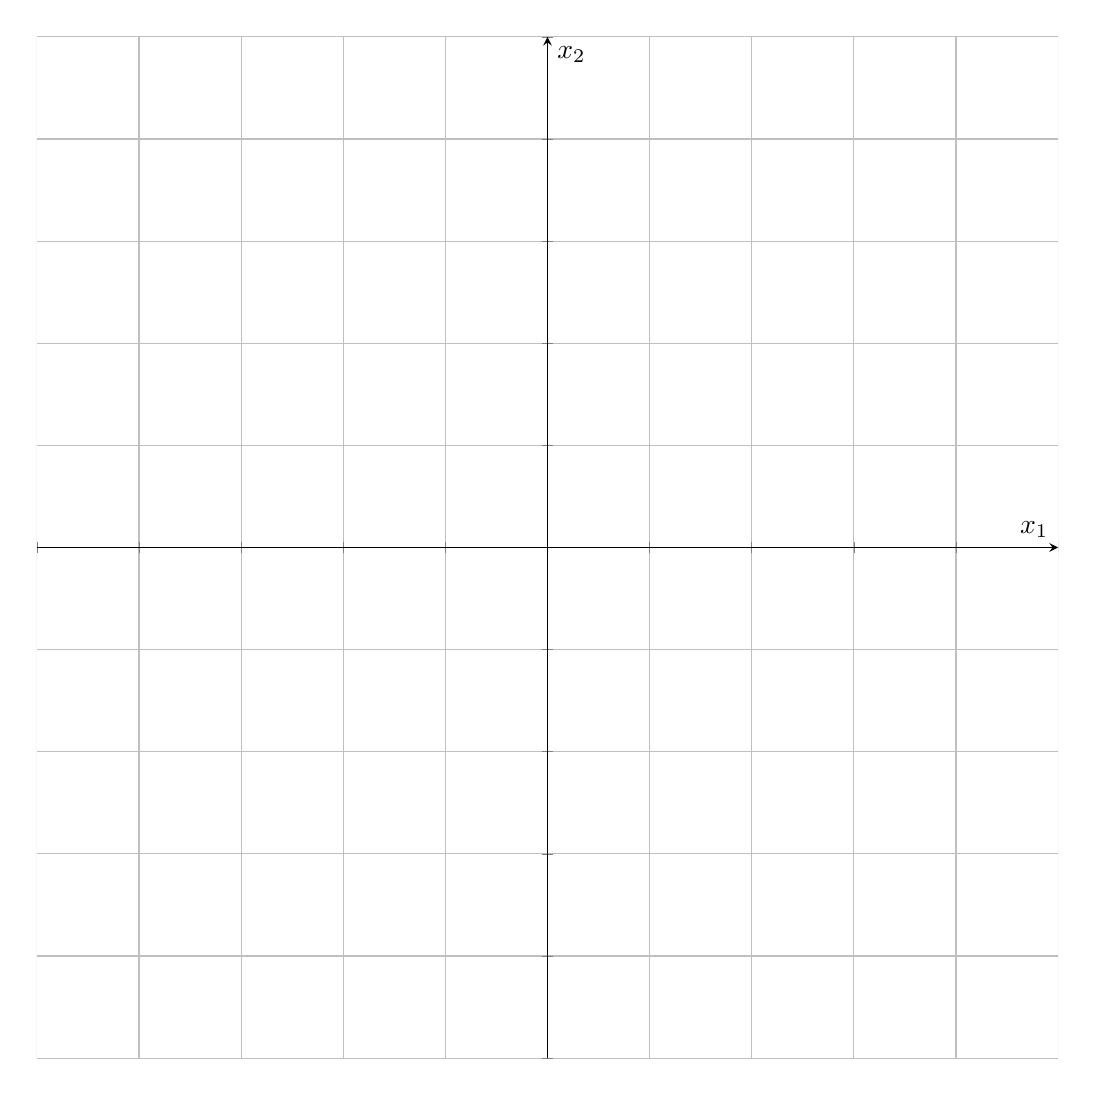
\begin{tikzpicture}
		\begin{axis}[
			height=1.2\textwidth,
			width=1.2\textwidth,
			axis lines = middle,
			xmin=-5, xmax=5, ymin=-5, ymax=5,
			xtick distance=1, ytick distance=1,
			xticklabels={}, yticklabels={,,},
			xlabel=\(x_1\), ylabel=\(x_2\),
			grid=major
		]
		\end{axis}
	\end{tikzpicture}
	\caption{Place (1.) here}
	\end{minipage}\hfill
	\begin{minipage}{0.3333\textwidth}
	\centering
	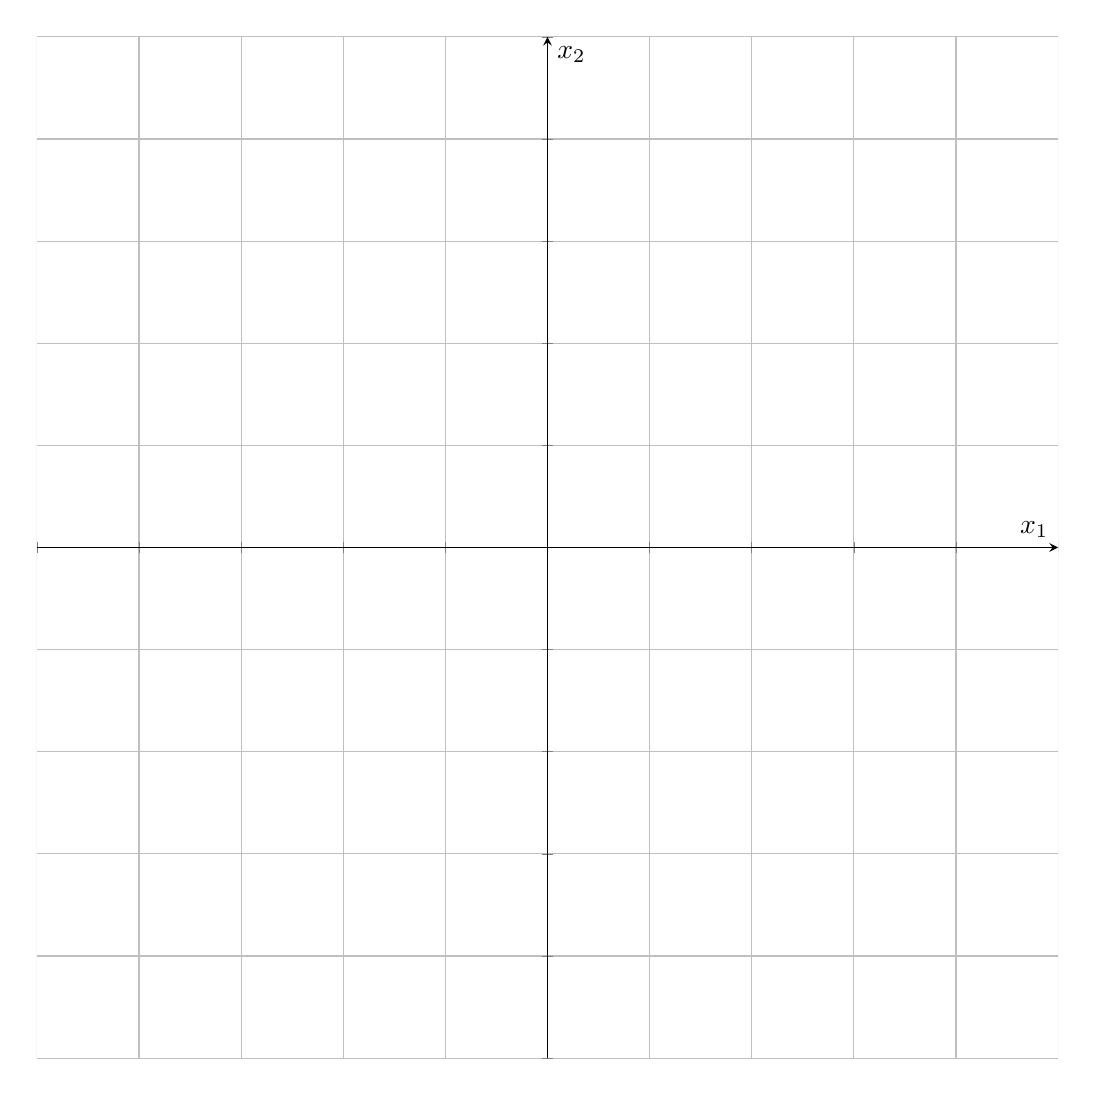
\begin{tikzpicture}
		\begin{axis}[
			height=1.2\textwidth,
			width=1.2\textwidth,
			axis lines = middle,
			xmin=-5, xmax=5, ymin=-5, ymax=5,
			xtick distance=1, ytick distance=1,
			xticklabels={}, yticklabels={},
			xlabel=\(x_1\), ylabel=\(x_2\),
			grid=major
		]
		\end{axis}
	\end{tikzpicture}
	\caption{Place (2.) here}
	\end{minipage}\hfill
	\begin{minipage}{0.3333\textwidth}
	\centering
	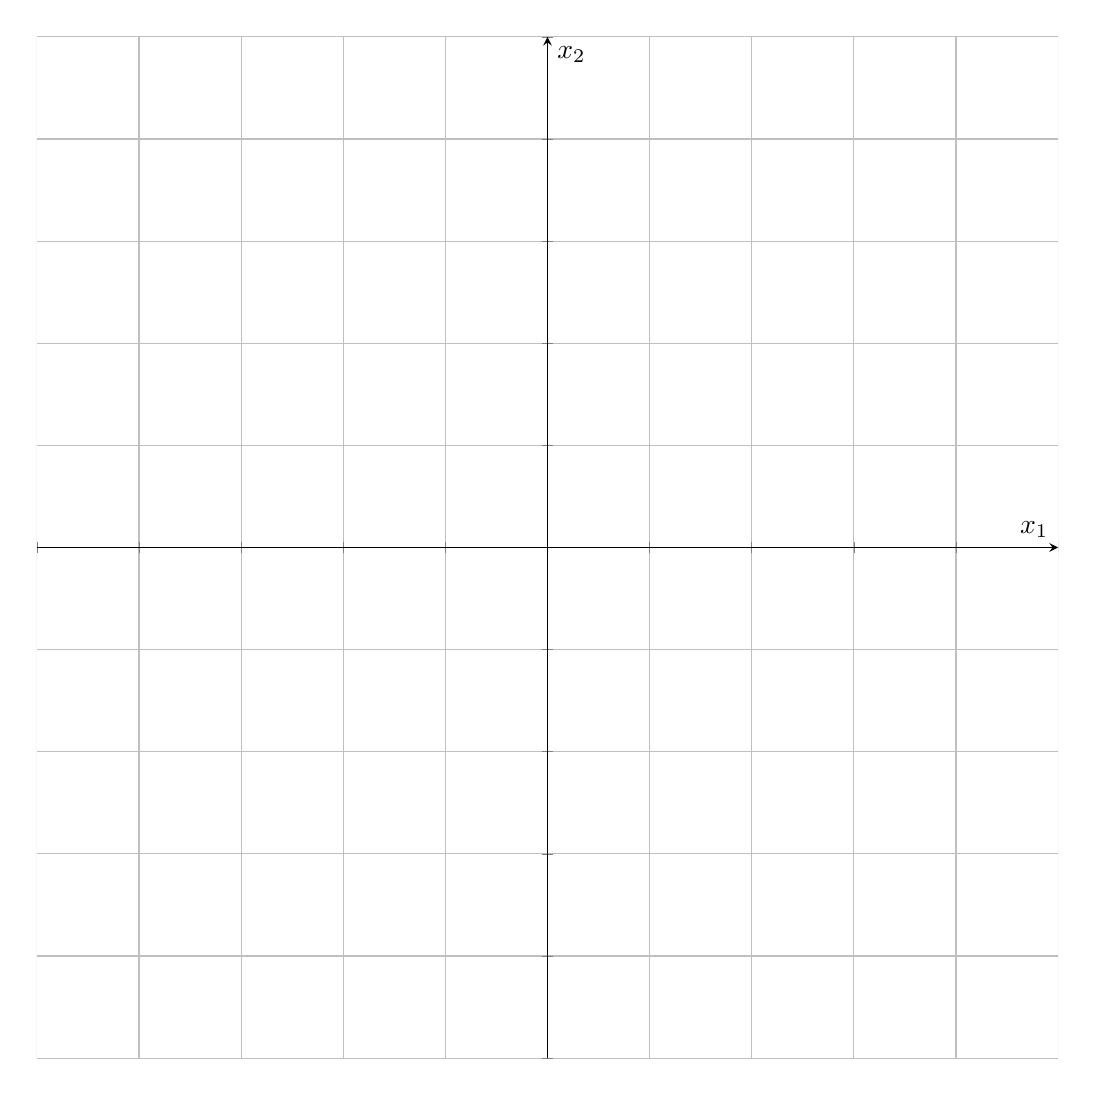
\begin{tikzpicture}
		\begin{axis}[
			height=1.2\textwidth,
			width=1.2\textwidth,
			axis lines = middle,
			xmin=-5, xmax=5, ymin=-5, ymax=5,
			xtick distance=1, ytick distance=1,
			xticklabels={}, yticklabels={},
			xlabel=\(x_1\), ylabel=\(x_2\),
			grid=major
		]
		\end{axis}
	\end{tikzpicture}
	\caption{Place (3.) here}
	\end{minipage}\hfill
\end{figure}

\subsection{Vector \& Matrix Equations}
\begin{mideea}{0.9}
	\[x_1\vec{a}_1 + x_2\vec{a}_2 + \cdots + x_n\vec{a}_n = \vec{b} \iff \begin{bmatrix} \vec{a}_1 & \vec{a}_2 & \cdots & \vec{a}_n\end{bmatrix}
	\begin{bmatrix}x_1 \\ x_2 \\ \vdots \\ x_n\end{bmatrix} = \vec{b}\]
	\centering \textit{The matrix equation \(A\vec{x} = \vec{b}\) and the vector equation} \(\sum_{k=1}^n x_k\vec{a}_k = \vec{b}\)\footnote{
	\(\sum_{k=1}^n x_k\vec{a}_k\) is a more compact way of writing out \(x_1\vec{a}_1 + x_2\vec{a}_2 + \cdots + x_n\vec{a}_n\).} \textit{have the same 
	solution set, and correspond to the same system.}
\end{mideea}

\begin{newactivity}
Consider the following questions. Determine whether \(\vec{v} \in \vspan\{\vec{b}_1, \vec{b}_2\}\), and find the approriate scalars that lead to the 
correct linear combination:
	\begin{enumerate}
		\item \(\vec{v} = \begin{bmatrix}1 \\ 5 \\ 8\end{bmatrix}\), \(\vec{b}_1 = \begin{bmatrix}3 \\ 6 \\ 2\end{bmatrix}\) and \(\vec{b}_2 =
		\begin{bmatrix}1 \\ 3 \\7\end{bmatrix}\). (\textit{Hint: consider using the definition of span provided above to set up a vector equation.})

		\item \(\vec{v} = \begin{bmatrix}1 \\ 5 \end{bmatrix}\), \(\vec{b}_1 = \begin{bmatrix}0 \\ 10 \end{bmatrix}\) and \(\vec{b}_2 = \begin{bmatrix}-3 
		\\ 0\end{bmatrix}\). (\textit{Hint: Can you solve this by inspection?})
	\end{enumerate} 
\end{newactivity}

\section{\centering Matrix Equations \& Solution(s) of a System (1.4 \& 1.5)}
\subsection{Matrix Equations}
\begin{mideea}{0.9}
\begin{enumerate}
\item Given \(A \in \mathbb{R}^{m \times n}\) and any \(\vec{b} \in \mathbb{R}^m\), \(A\vec{x} = \vec{b}\) is inconsistent if and only if the REF of 
\(\begin{bmatrix}A & | & \vec{b}\end{bmatrix}\), which we'll call \(\begin{bmatrix}U & | & \vec{d}\end{bmatrix}\), has a row in the form 
\[\begin{bmatrix}0 & 0 & \cdots & 0 & | & d\end{bmatrix}, d \ne 0.\] It then follows that in order for \(A\vec{x} = \vec{b}\) to always be consistent for any 
\(\vec{b} \in \mathbb{R}^m\), \(A\) must have a pivot in every row.

\item From \textbf{Main Idea \#2}, \(A\vec{x} = \vec{b}\) is consistent if and only if \(\vec{b} \in \vspan\{\vec{a}_1, \vec{a}_2, \dots, \vec{a}_n\}\) (the 
columns  of \(A\)).
\end{enumerate}
\end{mideea}

\begin{newactivity}
Consider the following questions.
\begin{enumerate}
	\item Using one of the two (equivalent) rules above, come up with an inhomogenous system that is inconsistent, and where no entry in \(A\) is 0.
	\item For the equation \(\begin{bmatrix}2 & 6 \\ 4 & 12\end{bmatrix}\begin{bmatrix}x_1 \\ x_2\end{bmatrix} = \begin{bmatrix}3 \\ 6\end{bmatrix}\), find
		the paramteric vector form to describe the solution set and ``sketch" it.
\end{enumerate}
\end{newactivity}
\begin{figure}[!h]
	\centering
	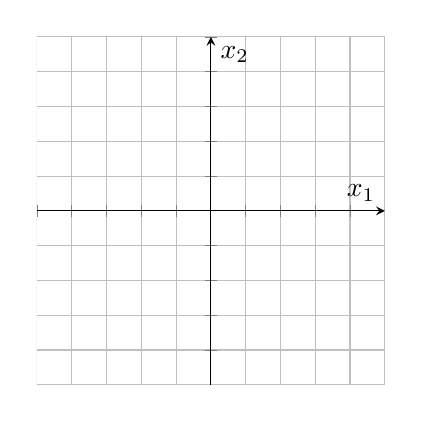
\begin{tikzpicture}
		\begin{axis}[
			height=6cm,
			width=6cm,
			axis lines = middle,
			xmin=-5, xmax=5, ymin=-5, ymax=5,
			xtick distance=1, ytick distance=1,
			xticklabels={}, yticklabels={,,},
			xlabel=\(x_1\), ylabel=\(x_2\),
			grid=major
		]
		\end{axis}
	\end{tikzpicture}
	\caption{Place (2.) here}
\end{figure}

\subsection{Homogenous and Inhomogenous Systems}
\begin{mideea}{0.9}
\[A\vec{x} = \vec{0} \ \text{has a nontrivial solution} \ \iff \text{free variables} \iff \rule{3cm}{0.15mm}\] \[\text{Homogenous system with free variables' solutions} \colon \vec{x} = t_1\vec{v}_1 + t_2\vec{v}_2 + \dots + t_k\vec{v}_k\] \[\text{Consistent inhomogenous system's solutions} \colon \vec{x} = \vec{v}_p +  t_1\vec{v}_1 + t_2\vec{v}_2 + \dots + t_k\vec{v}_k\]
(where \(k\) is the number of free variables and \(t_i \in \mathbb{R}\)).\footnote{If \(k=0\), meaning there are no free variables, then the trivial solution is the 
only solution, and the particular solution is the only solution for the consistent inhomogenous system.}
\end{mideea}

\begin{newactivity}
\begin{enumerate}
	\item Come up with a 2-by-3 matrix \(A\) that causes \(A\vec{x} = \vec{0}\) to have a nontrivial solution. (\textit{Hint: Can you do this by inspection only?
	Fill in the blank above to help you.}) 
\end{enumerate}
\end{newactivity}

\section{\centering Linear Indpendence (1.7)}
\begin{mideea}{0.9}
	A set of vectors \(\{\vec{v}_1, \vec{v}_2, \dots, \vec{v}_p \mid \vec{v}_i \in \mathbb{R}^n\}\) is linearly independent if and only if 
	\[c_1\vec{v}_1 + c_2\vec{v}_2 + \dots + c_p\vec{v}_p = \vec{0}, \ \text{with } c_i = 0, 1 \le i \le p\] is the only choice of scalars \(c_i\) satisfying the 
	vector equation. Equivalently, a set of vectors is linearly dependent if and only if there exists a vector in the set that could be written as a linear combination
	of the other vectors.
\end{mideea}

\begin{newactivity}
Answer the following questions.
\begin{enumerate}
\item Consider your answer from Section 1, subsesction 1.1 (\textbf{Span}). Which of the sets formed a linearly dependent set and which of them formed a 
	linearly independent set?
\item Consider a linearly dependent set \(\{\vec{v}_1, \vec{v}_2, \vec{v}_3\}\). Could \(\{\vec{v}_1, \vec{v}_3\}\) form a linearly independent set? Come up 
	with an example.
\item If \(\{\vec{v}_1, \vec{v}_2, \vec{v}_3\}\) forms a linearly independent set, is it possible that \(\{\vec{v}_1, \vec{v}_1 + \vec{v}_2, \vec{v}_3\}\) forms a
	linearly dependent set? (\textit{Hint: use the definition of linear independence to help you through this question.})
\end{enumerate}
\end{newactivity}

\section{\centering Linear Transformations (1.8, 1.9)}
\subsection{Introduction to Linear Transformations}
\begin{mideea}{0.9}
Any linear transformation \(T \colon \mathbb{R}^n \to \mathbb{R}^m\) could be represented through matrix-vector multiplication. A transformation \(T\) is 
linear if 
	\begin{enumerate}
		\item \(T(\vec{v} + \vec{u}) = T(\vec{v}) + T(\vec{u})\) for all vectors \(\vec{v}, \vec{u} \in \mathbb{R}^n\)
		\item \(T(c\vec{v}) = cT(\vec{v})\) for all \(c \in \mathbb{R}\) and \(\vec{v} \in \mathbb{R}^n\).
	\end{enumerate}
\end{mideea}

\begin{newactivity}
Given the information above, what should \(T(\vec{0})\) be for any linear transformation?
\end{newactivity}

\subsection{The Standard Matrix of a Linear Transformation}
\begin{mideea}{0.9}
\begin{enumerate}
\item The standard matrix of a linear transformation \(T \colon \mathbb{R}^n \to \mathbb{R}^m\) is the matrix
\[\begin{bmatrix}T(\vec{e}_1) & T(\vec{e}_2) & T(\vec{e}_3) & \dots & T(\vec{e}_n)\end{bmatrix}, \ \text{where} \ \{\vec{e}_i  \in \mathbb{R}^n \mid 1 \le i \le n\} \ \text{is the standard basis.}\]
\item \(T\) is one-to-one if and only if \(T(\vec{x}) = \vec{0}\) has the trivial solution only. Since \(T(\vec{x}) = A\vec{x}\), this tells us that \(T\) is one-to-one if 
	\(A\vec{x}=\vec{0}\) only has the trivial solution.
\item \(T \colon \mathbb{R}^n \to \mathbb{R}^m,\) with \(\vec{x} \mapsto A\vec{x}\), is onto if and only if the columns of \(A\) \rule{3cm}{0.15mm}.
\end{enumerate}
\end{mideea}

\begin{newactivity}
	\begin{enumerate}
		\item Find the standard matrix of the transformation \(T \colon \mathbb{R}^3 \to \mathbb{R}^2\) that projects everything down into the floor 	
		(discarding the third component of the vector). Is this transformation one-to-one? Is it onto?
		\item Find the standard matrix of the transformation \(T \colon \mathbb{R}^2 \to \mathbb{R}^3\) that embeds everything in \(\mathbb{R}^2\) into
		the ``floor" of \(\mathbb{R}^3\).
	\end{enumerate}
\end{newactivity}

\section{\centering Solutions}
\paragraph{Solutions to Activity 1}
\begin{enumerate}
	\item Any line that passes through the origin. Examples:
	\begin{figure}[!h]	
		\centering
		\begin{minipage}{0.5\textwidth}
		\centering
		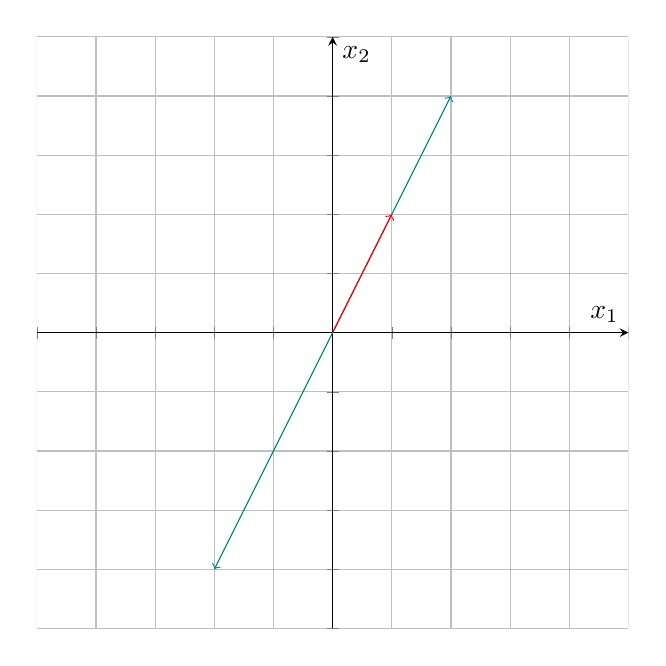
\begin{tikzpicture}
		\begin{axis}[
			height=0.75\textwidth,
			width=0.75\textwidth,
			axis lines = middle,
			xmin=-5, xmax=5, ymin=-5, ymax=5,
			xtick distance=1, ytick distance=1,
			xticklabels={}, yticklabels={,,},
			xlabel=\(x_1\), ylabel=\(x_2\),
			grid=major
		]
		\addplot[<->, color=teal, domain=-2:2, ] {2*x};
		\addplot[->, color=red, domain=0:1]{2*x};
		\end{axis}
	\end{tikzpicture}
	\caption{\(\vspan\left\{\begin{bmatrix}1 \\ 2\end{bmatrix}\right\}\)}
	\end{minipage}\hfill
		\begin{minipage}{0.5\textwidth}
		\centering
		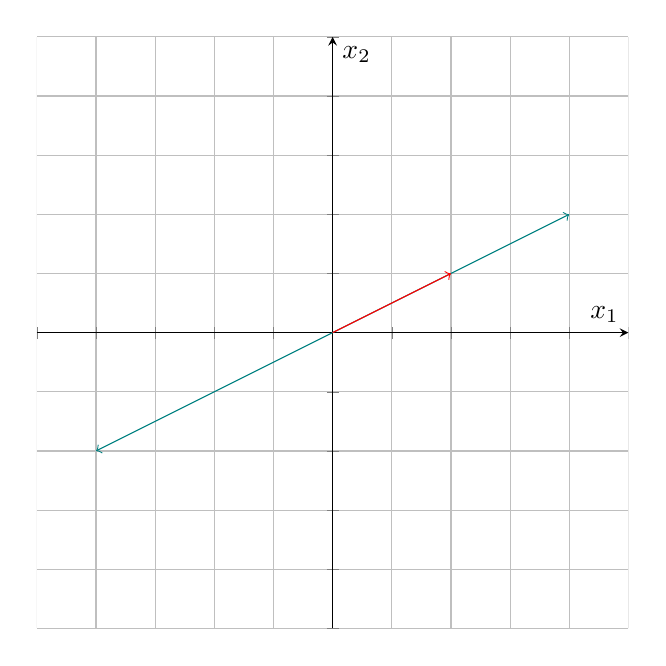
\begin{tikzpicture}
		\begin{axis}[
			height=0.75\textwidth,
			width=0.75\textwidth,
			axis lines = middle,
			xmin=-5, xmax=5, ymin=-5, ymax=5,
			xtick distance=1, ytick distance=1,
			xticklabels={}, yticklabels={,,},
			xlabel=\(x_1\), ylabel=\(x_2\),
			grid=major
		]
		\addplot[<->, color=teal, domain=-4:4, ] {0.5*x};
		\addplot[->, color=red, domain=0:2, ] {0.5*x};
		\end{axis}
	\end{tikzpicture}
	\caption{\(\vspan\left\{\begin{bmatrix}2 \\ 1\end{bmatrix}\right\}\)}
	\end{minipage}\hfill
	\end{figure}

\item Any set of two vectors that are in the span of each other. Examples:
	\begin{figure}[!h]	
		\centering
		\begin{minipage}{0.5\textwidth}
		\centering
		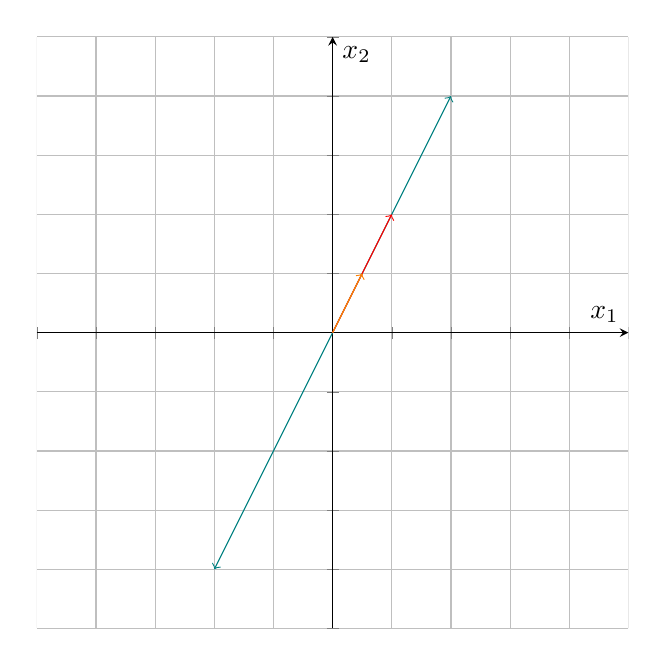
\begin{tikzpicture}
		\begin{axis}[
			height=0.75\textwidth,
			width=0.75\textwidth,
			axis lines = middle,
			xmin=-5, xmax=5, ymin=-5, ymax=5,
			xtick distance=1, ytick distance=1,
			xticklabels={}, yticklabels={,,},
			xlabel=\(x_1\), ylabel=\(x_2\),
			grid=major
		]
		\addplot[<->, color=teal, domain=-2:2] {2*x};
		\addplot[->, color=red, domain=0:1]{2*x};
		\addplot[->, color=orange, domain=0:0.5]{2*x};
		\end{axis}
	\end{tikzpicture}
	\caption{\(\vspan\left\{\begin{bmatrix}1 \\ 2\end{bmatrix}, \begin{bmatrix}0.5 \\ 1\end{bmatrix}\right\}\)}
	\end{minipage}\hfill
		\begin{minipage}{0.5\textwidth}
		\centering
		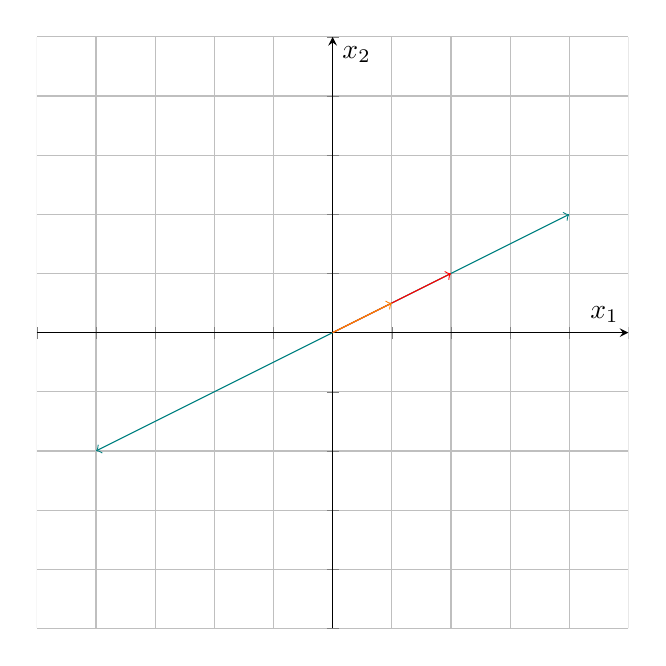
\begin{tikzpicture}
		\begin{axis}[
			height=0.75\textwidth,
			width=0.75\textwidth,
			axis lines = middle,
			xmin=-5, xmax=5, ymin=-5, ymax=5,
			xtick distance=1, ytick distance=1,
			xticklabels={}, yticklabels={,,},
			xlabel=\(x_1\), ylabel=\(x_2\),
			grid=major
		]
		\addplot[<->, color=teal, domain=-4:4, ] {0.5*x};
		\addplot[->, color=red, domain=0:2, ] {0.5*x};
		\addplot[->, color=orange, domain=0:1, ] {0.5*x};
		\end{axis}
	\end{tikzpicture}
	\caption{\(\vspan\left\{\begin{bmatrix}2 \\ 1\end{bmatrix}, \begin{bmatrix}1 \\ 0.5\end{bmatrix}\right\}\)}
	\end{minipage}\hfill
	\end{figure}
\item Any two linearly independent vectors. An example
	\begin{figure}[!h]
	\centering
	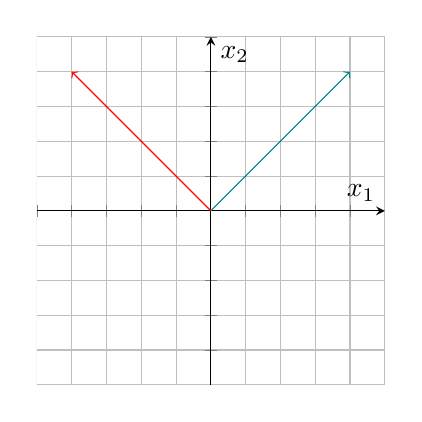
\begin{tikzpicture}
		\begin{axis}[
			height=6cm,
			width=6cm,
			axis lines = middle,
			xmin=-5, xmax=5, ymin=-5, ymax=5,
			xtick distance=1, ytick distance=1,
			xticklabels={}, yticklabels={,,},
			xlabel=\(x_1\), ylabel=\(x_2\),
			grid=major
		]
		\addplot[->, color=teal, domain=0:4]{x};
		\addplot[<-, color=red, domain=-4:0]{-x};		
		\end{axis}
	\end{tikzpicture}
	\caption{\(\left\{\begin{bmatrix}4 \\ 4\end{bmatrix}, \begin{bmatrix}-4 \\ 4\end{bmatrix}\right\}\)}
	\end{figure}

Intuitively, 2 linearly independent vectors define 2 ``new navigation directions" in the vector space, so we can move in 2 ``unique" directions (i.e., right and up, 
according to these two linearly independent vectors).
\end{enumerate}

\paragraph{Solutions to Activity 2}
\begin{enumerate}
\item Set the appropriate equation \[c_1\begin{bmatrix}3 \\ 6 \\ 2\end{bmatrix} + c_2\begin{bmatrix}1 \\ 3 \\ 7\end{bmatrix} = \begin{bmatrix}1 \\ 5 \\ 8\end{bmatrix}\] Then, realize that \[c_1\begin{bmatrix}3 \\ 6 \\ 2\end{bmatrix} + c_2\begin{bmatrix}1 \\ 3 \\ 7\end{bmatrix} = \begin{bmatrix}1 \\ 5 \\ 8\end{bmatrix} \iff \begin{bmatrix}3 & 1 \\ 6 & 3 \\ 2 & 7\end{bmatrix}\begin{bmatrix}c_1 \\ c_2\end{bmatrix} = \begin{bmatrix}1 \\ 5 \\ 8\end{bmatrix}\]
So, determine if the system is consistent or not. (If not, then there does not exists scalars \(c_1, c_2 \in \mathbb{R}\) that satisfy the vector equation.)
\[\left(\begin{array}{cc|c}3 & 1 & 1 \\ 6 & 3 & 5 \\ 2 & 7 & 8\end{array}\right) \sim \cdots \sim \left(\begin{array}{cc|c}1 & 0 & 0 \\ 0 & 1 & 0 \\ 0 & 0 & 1\end{array}\right)\]
We see that there is a pivot in the augmented column, so the system is inconsistent (i.e., there does not exists scalars \(c_1, c_2\) that allows for the two vectors \(\vec{b}_1, \vec{b}_2\) to be scaled and combined to get the vector \(\vec{v}\)). So, the answer is \textbf{no.}

\item Notice that if you scaled \(\vec{b}_1\) by \(\frac{1}{2}\) and divided \(\vec{b}_2\) by \(-\frac{1}{3}\) and combined the result of scaling them, you get the
vector \(\vec{v}\). So, \(\vec{v} \in \vspan\{\vec{b}_1, \vec{b}_2\}\). No row-reduction needed!
\end{enumerate}

\paragraph{Solutions to Activity 3}
\begin{enumerate}
\item It's easier to come up with an inconsistent inhomogenous system if we considered rule (2). All we have to do is find a set of vectors and one more that isn't 
in the span of that set of vectors! Look at the solution to Activity 2, Part 1 to see what I mean!
\item By inspection, the particular solution to this system is \(\vec{v}_p = \begin{bmatrix}1 \\ 1/6\end{bmatrix}\). (Verify this!). We know that the paramteric 
vector form of the solution of an inhomogenous system is in the form \[\vec{x} = \vec{v}_p + \vec{v}_n, \ \text{where } \vec{v}_n \text{ is any solution for } A\vec{x} = \vec{0}.\] By inspection, the general solution to the homogenous system would be \(\vec{x} = t\begin{bmatrix}1 \\ -3\end{bmatrix}\). So, the general
form for the solution to the inhomogenous system would be \[\vec{x} = \begin{bmatrix}1 \\ 1/6\end{bmatrix} + t\begin{bmatrix}1 \\ -3\end{bmatrix}.\]
(Another way to solve this problem would be to simply row-reduce the augmented matrix.)
\begin{figure}[!h]
	\centering
	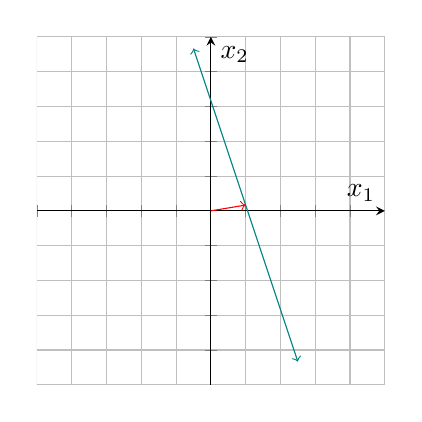
\begin{tikzpicture}
		\begin{axis}[
			height=6cm,
			width=6cm,
			axis lines = middle,
			xmin=-5, xmax=5, ymin=-5, ymax=5,
			xtick distance=1, ytick distance=1,
			xticklabels={}, yticklabels={,,},
			xlabel=\(x_1\), ylabel=\(x_2\),
			grid=major
		]
		\addplot[<->, color=teal, domain=-1.5:1.5]({x+1}, {1/6 - 3 * x});
		\addplot[->, color=red, domain=0:1]{0.1667*x};
		\end{axis}
	\end{tikzpicture}
	\caption{The red vector is \(\vec{v}_p\), and the blue line represents \(t\begin{bmatrix}1 \\ -3\end{bmatrix}\)}
\end{figure}
\end{enumerate}

\paragraph{Solution to Activity 4}
\begin{enumerate}
	\item For the \textbf{Main Idea} box, the blank should say: \textit{linear dependent}.
	\item Coming up with 2-by-3 matrix \(A\) that causes \(A\vec{x} = \vec{0}\) to have a non-trivial solution implies that the columns form a linearly 
		\emph{dependent} set. (To see why, go back to the definition of linear dependence.) This becomes simple now: Find any two vectors, take a random 
		linear combination of them, set the resulting vector as the third column of the matrix, and you're done. If you understood this, then you've practicaly 
		understood the idea behind this question.
\end{enumerate}

\paragraph{Solution to Activity 5}
\begin{enumerate}
	\item The first two formed a linearly dependent set, while the last one formed a linearly dependent set. This is because, in the first two example, it was 
		possible two write one vector as a linear combination of the other. However, this is not possbile in the last part. 
	\item Sure; it's possible. The simplest example is \[\left\{\begin{bmatrix}0 \\ 0 \end{bmatrix}, \begin{bmatrix}1 \\ 0 \end{bmatrix}, \begin{bmatrix}0 \\ 1\end{bmatrix}\right\}\]
	\item This is impossible. One way to show this is to show that no vector can be represented as a linear combination of the other vectors (as I showed in 
		the PLUS session.) An easier way is to go back to the definition of linear independence. We're asking, what are the possible scalars \(c_1, c_2, c_3\) 
		such that \[c_1\vec{v}_1 + c_2(\vec{v}_1 + \vec{v}_2) + c_3\vec{v}_3 = \vec{0}\] 
		But then 
		\[c_1\vec{v}_1 + c_2(\vec{v}_1 + \vec{v}_2) + c_3\vec{v}_3 = \vec{0} \implies c_1\vec{v}_1 + c_2\vec{v}_1 + c_2\vec{v}_2 + c_3\vec{v}_3 = 
		\vec{0} \implies (c_1 + c_2)\vec{v}_1 + c_2\vec{v}_2 + c_3\vec{v}_3 = \vec{0}\]
		Now we have to remember something very important: \(\{\vec{v}_1, \vec{v}_2, \vec{v}_3\}\) forms a linearly \emph{independent} set, meaning
		\[0\vec{v}_1 + 0\vec{v}_2 + 0\vec{v}_3 = \vec{0}\] is the only possible situation. But see, we've got something quite similar to that up there. This 
		means that the only possible situation is
		\[\underbrace{(c_1 + c_2)}_{0}\vec{v}_1 + \underbrace{c_2}_{0}\vec{v}_2 + \underbrace{c_3}_{0}\vec{v}_3 = \vec{0}\] Is this possible? What 
		values of \(c_1, c_2, c_3\) satisfy
		\begin{align}
			c_1 + c_2 &= 0 \\
			c_2 &= 0 \\
			c_3 &= 0
		\end{align}
		Well, we see that \(c_3 = 0\), and \(c_2 = 0\), and \(c_1 + c_2 = 0 \implies c_1 = -c_2\). But \(c_2 = 0\), which means that \(c_1 = 0\) as well.

		Basically, we went back to the original defiintion of what it means to be linearly independent/dependent, and from there we've reached something we 
		know (we know that \(\{\vec{v}_1, \vec{v}_2, \vec{v}_3\}\) forms a linearly \emph{independent} set). Finally, we found out that the only possible 
		choices of \(c_1, c_2, c_3\) is 0. Therefore, the new set is also necessarily linearly independent.
\end{enumerate}

\paragraph{Solution to Activty 6}
	\[T(\vec{0}) = \underbrace{T(0 \cdot \vec{v})}_{\text{for any} \ \vec{v} \in \mathbb{R}^n} = 0 \cdot T(\vec{v}) = \vec{0}\]

\paragraph{Solution to Activity 7}
	\begin{enumerate}
		\item The mapping here is \[\begin{bmatrix}x_1 \\ x_2 \\ x_3\end{bmatrix} \mapsto \begin{bmatrix}x_1 \\ x_2\end{bmatrix}\] It is easy to see that 
			this transformation is onto, because for any vector \(\begin{bmatrix}x_1 \\ x_2\end{bmatrix} \in \mathbb{R}^2\), I can choose a vector living
			in \(\mathbb{R}^3\) such that applying that transformation takes me to \(\begin{bmatrix}x_1 \\ x_2\end{bmatrix}\). Basically, every vector in 
			\(\mathbb{R}^2\) gets hit. So the transformation is onto. 

			However, the transformation is \emph{not} one-to-one. To see why, take two vectors \(\begin{bmatrix}x_1 \\ x_2 \\ b_1\end{bmatrix}\) and 
			\(\begin{bmatrix}x_1 \\ x_2 \\ b_2\end{bmatrix}\) with \(b_1 \ne b_2\). The transformation maps them to the same vector, so it's not one-to-
			one.
			
			For the standard matrix: \[\begin{bmatrix}T(\vec{e}_1) & T(\vec{e}_2) & T(\vec{e}_3)\end{bmatrix} = \begin{bmatrix}1 & 0 & 0 \\ 0 & 1 & 0 \end{bmatrix}\]
		\item \[\begin{bmatrix}T(\vec{e}_1) & T(\vec{e}_2)\end{bmatrix} = \begin{bmatrix}1 & 0 \\ 0 & 1\\ 0 & 0\end{bmatrix}\] Is this transformation 
			onto? Is it one-to-one?
	\end{enumerate}
\end{document}